\documentclass[../main.tex]{subfiles}

\begin{document}
    \chapter{The Local Adaptive Network}\label{chap:loadnetwork}
    
    In this chapter we introduce our novel Local Adaptive Network that is able to
    discover the image parts more responsible of the domain shift and to perform a
    tailored adaptation across source and target samples.

    This technique builds upon three methods:
    \begin{enumerate}
        \item We employ a modification of Grad-CAM~\cite{gradcam} to generate what we call \textit{domainness maps},
            which tell us on a per-feature-map basis which regions in the image are discriminative between
            source and target domains.
        \item Spatial Pyramid Pooling~\cite{sppooling} is used to perform pooling at multiple levels in a parallel fashion.
            This can be useful when localization of the object in the image is an issue.
            It also generates fixed-length representations regardless of the input size.
        \item Inspired by the Multiplicative Fusion approach presented in~\cite{multfusion}, we combine the information
            provided by the domainness maps with that coming from the feature maps. The maps inhibit domain-specific regions
            (regions that are discriminative for the two domains) and enhance domain-generic regions, thereby reducing the
            domain shift between source and target.
    \end{enumerate}
    
    In the following, we review each of these components and we explain how they have been combined for our
    Local Adaptive Network.

    \section{Grad-CAM}

    \paragraph{Motivation}

    Grad-CAM (Gradient-weighted Class Activation Mapping)~\cite{gradcam} is a method for visualizing the spatial locations
    in an image that contributed the most to the CNN's classification choice.
    The technique is applicable to a wide variety of tasks, ranging from image captioning to visual question answering to
    reinforcement learning, and also to a wide variety of CNN architectures. \\
    Grad-CAM was designed as a visualization tool to better understand how CNNs reason and to improve
    their interpretability, which is a fundamental property to have for AI systems that wants to be deployed
    in the real world. In the context of this thesis work, we use this technique to visualize the spatial grounding of
    domain shift: looking for the regions more or less responsible for the difference across domains.

    \paragraph{How it works}

    Although visualizations can be extracted at any layer of the hierarchy, we opted for the last convolutional layer,
    because it is the best compromise between high-level semantics and spatial localization.
    The former is a general property of deep learning models: the further the layer from the input,
    the more high-level and meaningful the features extracted are. The latter is a property of
    convolutional feature maps, which are designed to retain as much spatial information as possible about
    the input. Fully-connected layers down the hierarchy do not have this property. \\
    The high-level structure of the method can be seen in the following figure:

	\begin{figure}[h!]
        \centering{}
        \makebox[\linewidth][c]{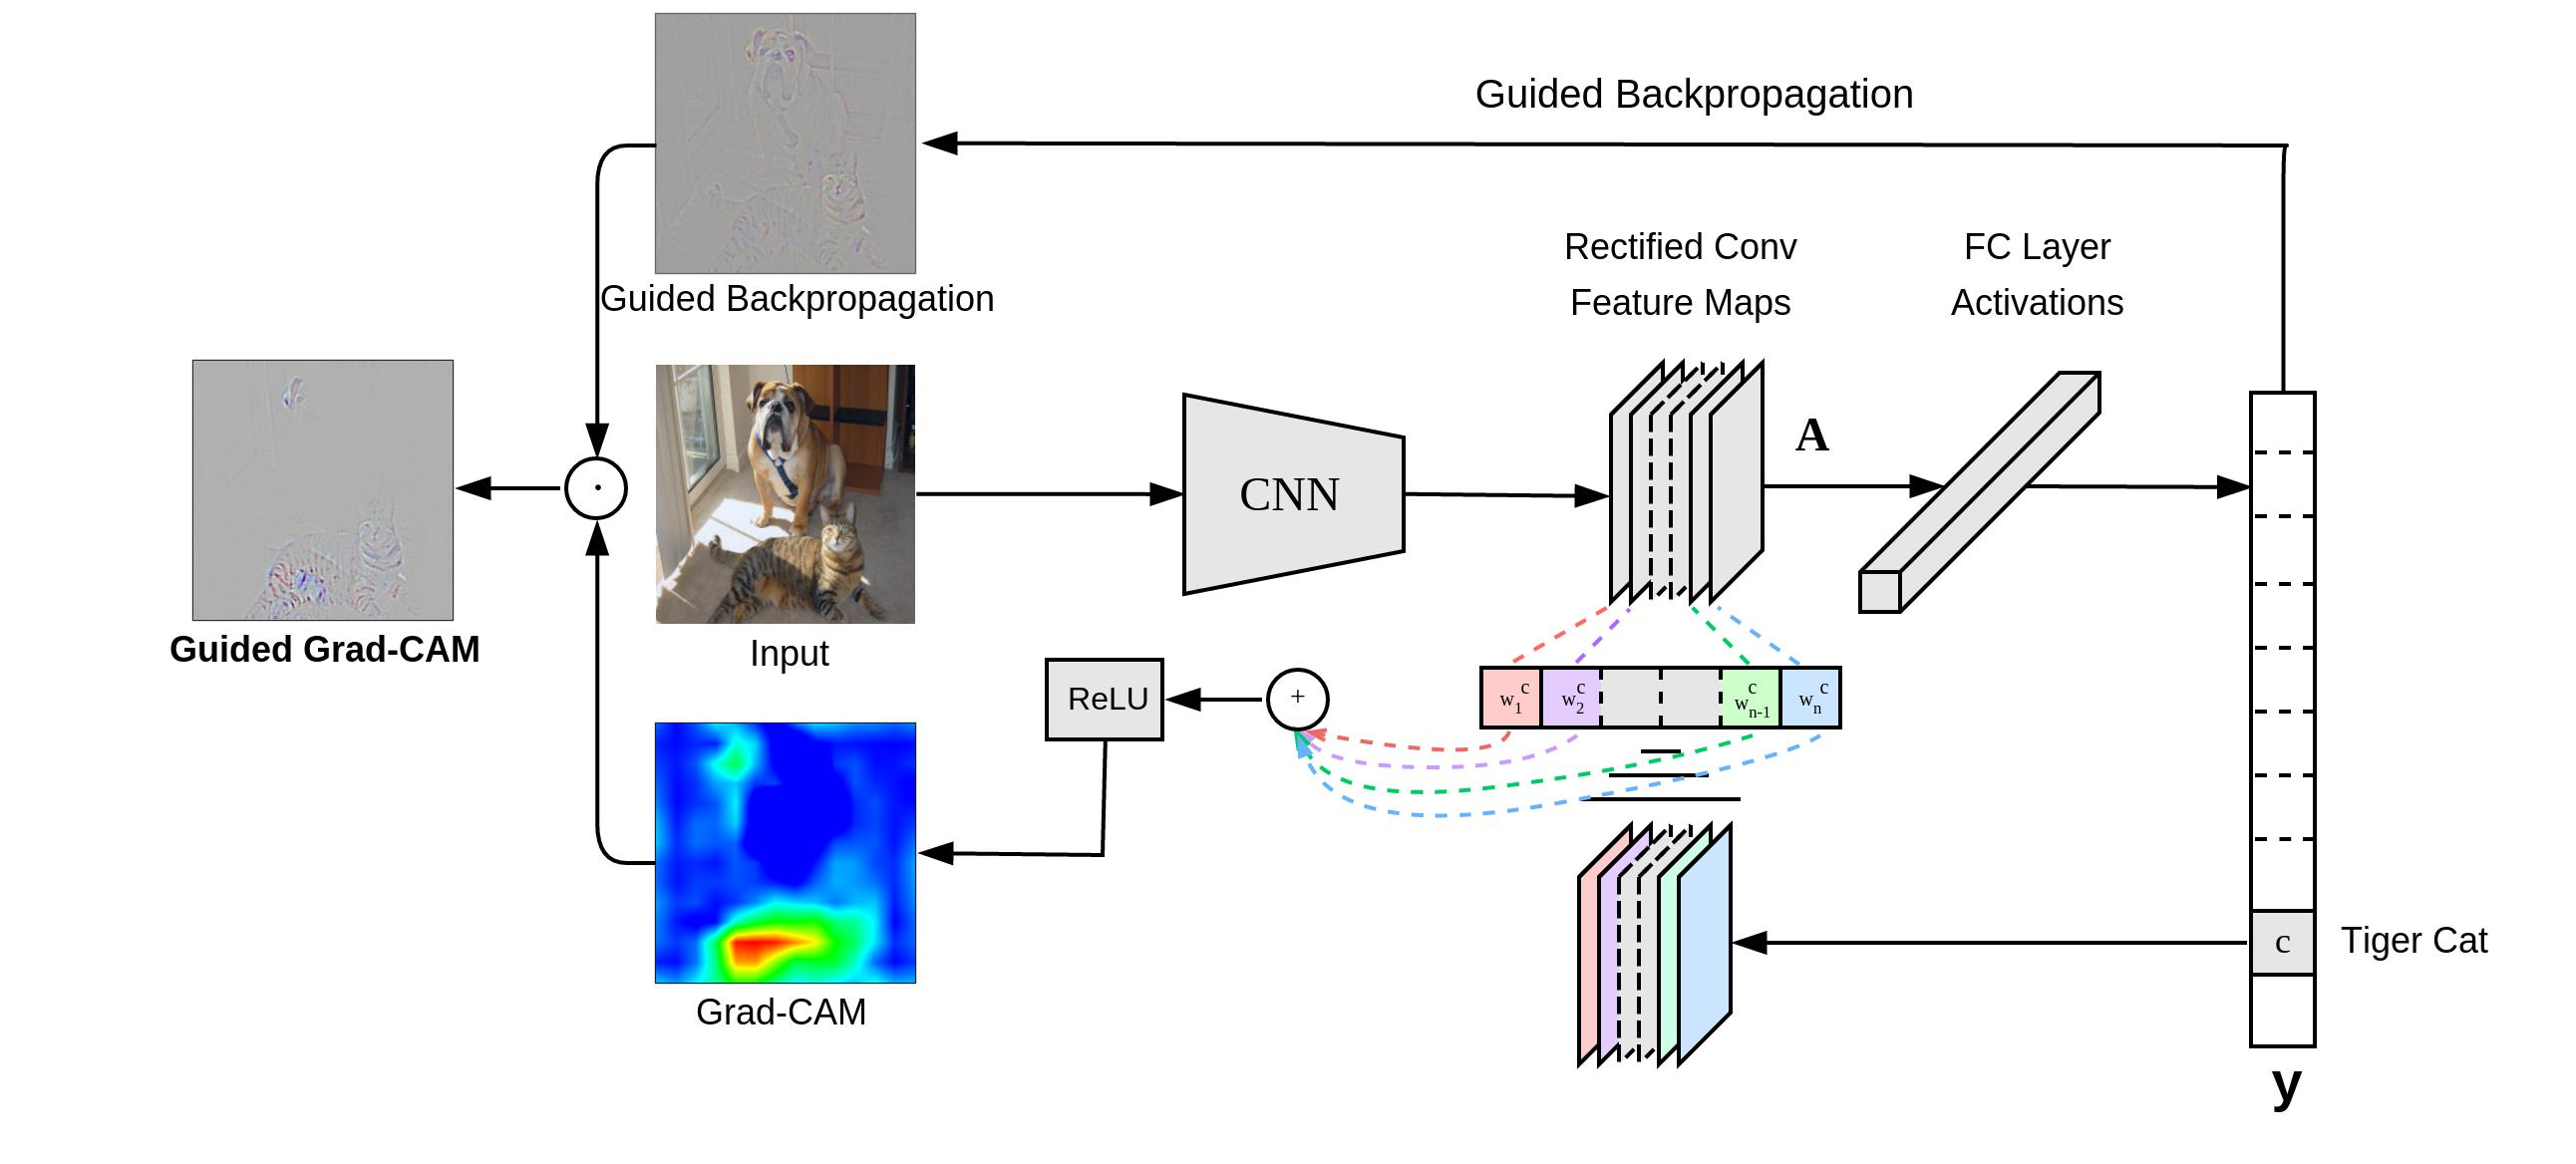
\includegraphics[width=1.4\linewidth]{img/gradcam-architecture.png}}
	    \caption{Grad-CAM Architecture, taken from~\cite{gradcam}}\label{fig:gradcam-architecture}
	\end{figure}

    Basically, the input image is forward propagated through the network in order to compute the softmax scores
    of the last layer, which we call $y^{c} = f(x)$, where $f()$ is the input-output network mapping.
    If we were training the network, at this point we would have computed the gradients of the
    last layer neurons with respect to some loss function, like cross-entropy. Instead, in Grad-CAM, we manually
    create these gradients. In particular, we set them to one for the neuron corresponding to the class of interest,
    while all the other neurons are set to zero.
    $$ \frac{\partial y^{c}}{\partial \theta_{output}} = [0, 0, \ldots , 1, 0, 0, \ldots] $$
    Then, we backward propagate these gradients through the network until
    the last convolutional layer, where the Grad-CAM map is created. Assuming that the last convolutional layer feature maps are
    in $ \mathbb{R}^{K \times H \times W} $, where $H$ and $W$ are respectively the height and the width of each feature
    map, and $K$ is the number of feature maps (depth). The map that will be generated is thus in $\mathbb{R}^{H \times W}$.
    The generation procedure has multiple steps:
    \begin{enumerate}
        \item Compute the weight of each feature maps. We want a number measuring how much each filter contributed to
            the final score. It is therefore natural to compute this number as the derivative of the output gradients
            with respect to the weights of the filter. These derivatives are then global average pooled in order to get
            a single number:
            \begin{equation}
                w_{k}^{c} = \frac{1}{Z} \sum_{i = 1}^{h} \sum_{j = 1}^{w} \frac{\partial y^{c}}{\partial F_{i, j}^{k}},
            \end{equation}
            here $w_{k}^{c}$ is the weight of feature map $k$ with respect to target class $c$, while $F$ is the feature map
            itself. We can see that the derivative is positive if an increase of the value of the pixel $F_{i, j}^{k}$ yields
            an increase of the value of $y^{c}$.
        \item The Grad-CAM map is obtained by performing a rectified weighted linear combination of the forward feature maps:
            \begin{equation}\label{eq:gradcamMaps}
                M^{c} = ReLU \left( \sum_{k = 1}^{K} w_{k}^{c} F^{k} \right) \in \mathbb{R}^{H \times W}
            \end{equation}
    \end{enumerate}
    The $ReLU()$ function simply set to zero all the negative values. The Grad-CAM technique uses this function to retain only
    the values that have a \textit{positive} influence on the class decision.
    Once the Grad-CAM map is produced, it is then upsampled to the pixel space using bi-linear interpolation, then a heatmap
    is generated from the values and the heatmap is point-wise multiplied with the output of the Guided-BackPropagation
    procedure~\cite{guidedbackprop}, to produce the final result called Guided-GradCAM.\@

    \subsection{Grad-CAM for domain localization}\label{subsec:gradcam-domainness}

    To perform domain localization with Grad-CAM, we replaced the 1000-units softmax of ImageNet CNNs with a single sigmoid
    unit, and we fine-tuned the network to perform a binary classification between source and target samples. Our rationale is
    that by applying Grad-CAM to this binary network we are able to determine which regions
    in the image are \textit{domain-specific} (information contained only in one domain and not in the other) or
    \textit{domain-generic} (information shared between domains). Having this clue on a \textit{per-feature-map} basis,
    we are able to make source and target more similar at the representational level, by removing domain-specific locations and
    enhancing domain-generic ones. Figure~\ref{fig:domain-shift-office} depicts two sample images along with their domain-specific and
    domain-generic heatmaps, obtained by summing the per-feature-map activations over depth. \\

    \begin{figure}[h!]
        \centering

        \begin{subfigure}{\linewidth}
        	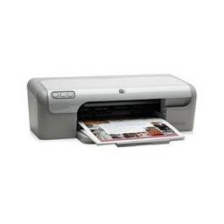
\includegraphics[width=.3\linewidth]{img/a1.png}\label{fig:amazon-1}\hfill
        	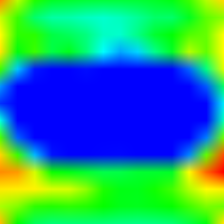
\includegraphics[width=.3\linewidth]{img/a-ad-a-1.png}\label{fig:amazon-amazon-1}\hfill
            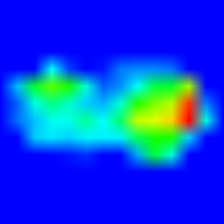
\includegraphics[width=.3\linewidth]{img/a-ad-d-1.png}\label{fig:amazon-dslr-1}
        \end{subfigure}

        \begin{subfigure}{\linewidth}
        	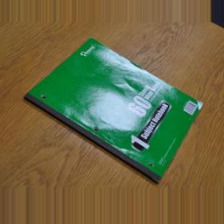
\includegraphics[width=.3\linewidth]{img/d1.png}\label{fig:dslr-1}\hfill
        	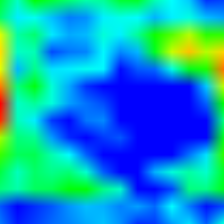
\includegraphics[width=.3\linewidth]{img/d-ad-d-1.png}\label{fig:dslr-dslr-1}\hfill
            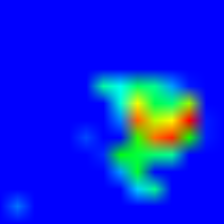
\includegraphics[width=.3\linewidth]{img/d-ad-a-1.png}\label{fig:dslr-amazon-1}
        \end{subfigure}

        \caption{Examples of domainness maps. Both rows have: (left) original image, (center) domain-specific map,
            (right) domain-generic map. We can see that the domain-specific map captures information contained in one domain
            but not in the other, in this case the background. Domain-generic maps instead captures information shared between
            domains, in this case the objects themselves.}\label{fig:domain-shift-office}
	\end{figure}

    Our domainness maps are actually generated using a subpart of the full Guided-GradCAM procedure.
    In particular, we used only Grad-CAM maps (without Guided-BackPropagation), and we retained the full
    \textit{per feature-map activations}, instead of summing them across depth.
    Namely, in our method, equation~\ref{eq:gradcamMaps} becomes:
    \begin{equation}\label{eq:gradcamDomain}
        M^{c} = ReLU \left( w_{k}^{c} F^{k} \right) \in \mathbb{R}^{K \times H \times W}
    \end{equation}
    That is, instead of summarizing into a single map, we retain information about how each filter contributed to the decision
    of the class. This is crucial, as it enables us to enhance and inhibit filters with a greater precision.
    
    \section{Spatial Pyramid Pooling}\label{sec:spatialpyramidpooling}
    \paragraph{Motivation}
    As explained in Section~\ref{subsec:convnets}, the max pooling operation is the most popular
    choice to perform dimensionality reduction in CNNs. Max pooling is a sliding window of a certain size in which for each window,
	the pixel with the maximum value is taken as output.
	Other summary statistics were employed in the literature, such as average pooling or sum pooling, but max pooling was found to
	work best in the context of object recognition~\cite{maxpooling}.
    After the last pooling layer, the resulting 3D tensor of dimension $C \times H \times W$ is flattened into a 1D tensor,
    and a series of fully-connected layers is placed on top of this layer. The are at least two problems with this architecture:
    \begin{itemize}
        \item Convolutional layers can deal with images of different sizes, but they will also produce outputs of different sizes. Fully-connected
            layers instead, only accept inputs of fixed size. Thus, the previous architecture cannot exploit this strength of convolutional layers.
        \item The designer should carefully choose the dimension of the pooling layers because, as we have seen in our experiments, this can have
            a major impact on the overall performance of the model. In particular we have seen that the last pooling operation is of particular
            importance when the object is translated or scaled by a large amount of pixels.
    \end{itemize}
    
    \paragraph{SPP-Net}
    Spatial Pyramid Pooling (SPP) is a method that was used extensively by the computer vision community before the deep learning revolution.
    This paper~\cite{sppooling} introduced the technique in the context of CNNs. Basically, a Spatial Pyramid Pooling operation
    is composed by multiple max pooling operations performed at different window sizes and then concatenated together in the depth dimension.
    This seemingly simple modification of the standard pooling layer has profound implications, such that:

    \begin{itemize}
        \item With a SPP layer as the last layer before the MLP, the network can take in input images of arbitrary sizes, scales and aspect ratios.
        \item The network is much more robust to translation and scaling of the input, because a pooling done at multiple levels is much able to capture
            such variations.
        \item The authors shown a small but consistent classification accuracy improvement over a large range of architectures and datasets.
    \end{itemize}

    Figure~\ref{fig:sppnet} is a depiction of how this layer works. 
    \begin{figure}[h!]
        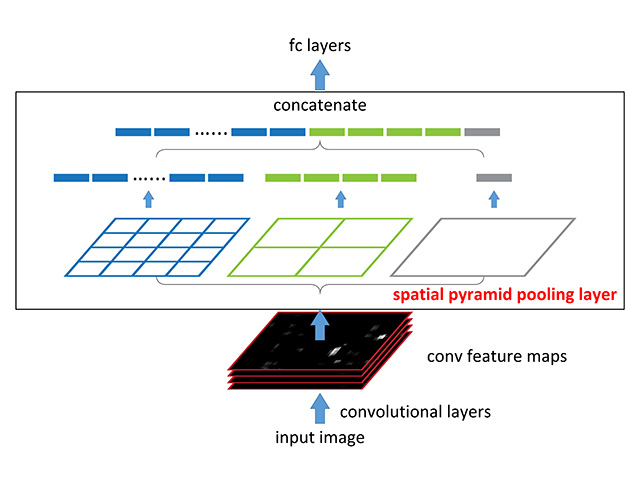
\includegraphics[width=\linewidth]{./img/sppnet.png}
        \caption{Spatial Pyramid Pooling layer. Image taken from:~\cite{sppooling}}\label{fig:sppnet}
    \end{figure}
    
    The pooling operation employed at each level is slightly different from the
    one we have described before. In particular, the one used here is called \textit{Adaptive Pooling}: instead of choosing the window size and the
    stride, we directly choose the output dimensions we want (say $n \times n$). From this, the window and the stride are automatically computed
    as $window = \ceil*{\frac{a}{n}}$ and $stride = \floor*{\frac{a}{n}}$, where $a$ is the dimension of the last conv layer feature maps. As a
    practical example, the VGG16 network~\cite{vgg16} last conv layer feature maps have dimension $512 \times 14 \times 14$\footnote{these are
    the output dimensions when the input image is $224 \times 224$. For bigger (smaller) images, $a$ would be greater (less) than $14$.
    However, using adaptive pooling, the output dimension will be $512 \times 4 \times 4$ regardless of the input size.}.
    If we want an adaptive max pooling of dimension $(4 \times 4)$, the window and the stride are computed as
    $window = \ceil*{\frac{14}{4}} = 4$ and $stride = \floor*{\frac{14}{4}} = 3$. Figure~\ref{fig:sppnet} has a SPP layer with three levels:
    $(4 \times 4) (2 \times 2) (1 \times 1)$. We can easily compute the (fixed) output dimension of this layer. For instance, with the VGG16
    network, the output size is: $(512*4*4) + (512*2*2) + (512*1*1) = 10752$, so we can place a fully-connected layer on top of this SPP and
    we can be sure that the dimension will be the same regardless of the input size. \\

	During our experiments we observed that the size of the window in the pooling operation is an important factor to take care of
	when dealing with a domain shift problem. Usually, one takes whatever dimension was chosen for the baseline network (AlexNet or VGG)
	and keeps it fixed. However, we adopted the original SPP strategy with the aim of testing different window sizes and we effectively
	verified that results can vary significantly based on this parameter. As a consequence, we believe that this is an important factor
    when dealing with learning across domains, and it cannot be considered simply fixed. The experiments empirically proved this intuition
    showing that this is a parameter that has to be carefully optimized.

    \section{Multi-cue Multiplicative-Fusion}\label{sec:load-network}
    \paragraph{Motivation}
    Learning by combining multiple information is one of the hallmarks of human intelligence and it is an important ability for any artificial
    agent. Many works has been dedicated to techniques for the integration of multiple cues. In particular, two approaches has been proposed in~\cite{multfusion},
    starting from CNN architectures in the context of action recognition.
    The first technique, which they called \textit{Feature Amplification},
    consists in an element-wise (hadamard) product between two sources of information: the first was the CNN feature maps and the second
    was the optical flow~\cite{opticalflow} information. The rationale was that through the multiplication, CNN feature maps information
    would detect important features for the action recognition task, and optical flow information would amplify (cancel out) important regions
    in the feature maps with respect to the task of detecting motion.
    The second method, named \emph{Multiplicative Fusion}, combines
    the feature maps coming from two different CNNs into a merged representation which is then propagated through the fully-connected layers.
    In particular, a new layer linearly combines the feature maps and the coefficients of the combination are considered as learnable parameters.
    Figure~\ref{fig:multfusion} shows the multiplicative fusion architecture.

    \begin{figure}[h!]
        \centering{}
        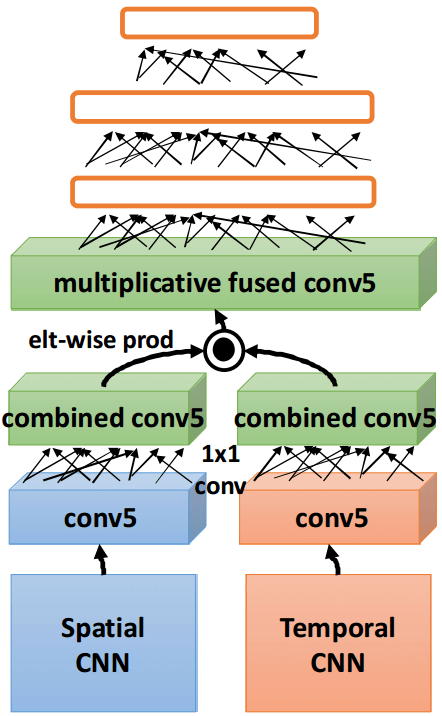
\includegraphics[width=.5\linewidth]{./img/multfusion.png}
        \caption{Multiplicative-Fusion architecture. Image taken from~\cite{multfusion}}\label{fig:multfusion}
    \end{figure}

    \subsection{Local Adaptive Convolutional Neural Network}
    Before introducing the details of our Local Adaptive Network (LoAd CNN) let's briefly recap our domain adaptation task and setting.
    We have two datasets which were drawn
    from two different distributions: the \textit{source} dataset $(X_{s}, Y_{s})$ was drawn from $P_{s}(X, Y)$, and the \textit{target}
    dataset $(X_{t})$ was drawn from $P_{t}(X)$, with $P_{s} \neq P_{t}$. Our learning task is to design a model that learns how to infer
    $Y_{t}$ given $(X_{s}, X_{t}, Y_{s})$. \\
    Our method can be summarized in the following way:
    \begin{enumerate}
        \item We train a CNN with a binary classifier on top of it to discriminate between source and target samples. The source samples are
            assigned a label of $0$, and the target samples a label of $1$. The CNN ends with a single sigmoid unit, which outputs the
            probability of the sample being a target sample:
            $$ P(Y = 1 | X) = \hat{y} $$
            This model is trained using the binary-cross-entropy loss function and stochastic gradient descent. Note that we are in the unsupervised
            domain adaptation setting and the procedure is completely agnostic of the target object labels.
        \item We use the Grad-CAM technique on the binary domain classification network to generate activation maps\@. In particular,
            for each image, we generate a domainness map of the regions that would make the classifier change its decision, from source to target or
            vice-versa. The activations are of the last convolutional layer, which has a more compact and meaningful representation, as the author
            of Grad-CAM also pointed out.
        \item The domainness maps are integrated into a final CNN that performs object classification on the source data. The final architecture can be seen in figure~\ref{fig:dmf-architecture}.
            From the input layer to the last convolutional layer, the architecture is the same as a standard CNN\@. Then, the output
            feature maps are duplicated: one copy is kept as in its original form, the other is multiplicatively fused with the domainness map.
            We use Spatial Pyramid Pooling for each of the two branches, motivated by our discussion in Section~\ref{sec:spatialpyramidpooling}.
            The two branches are then recombined by concatenation producing an enriched feature with an highlight on the domain generic parts of the images.
    \end{enumerate}

    \begin{figure}[h!]
        \centering{}
        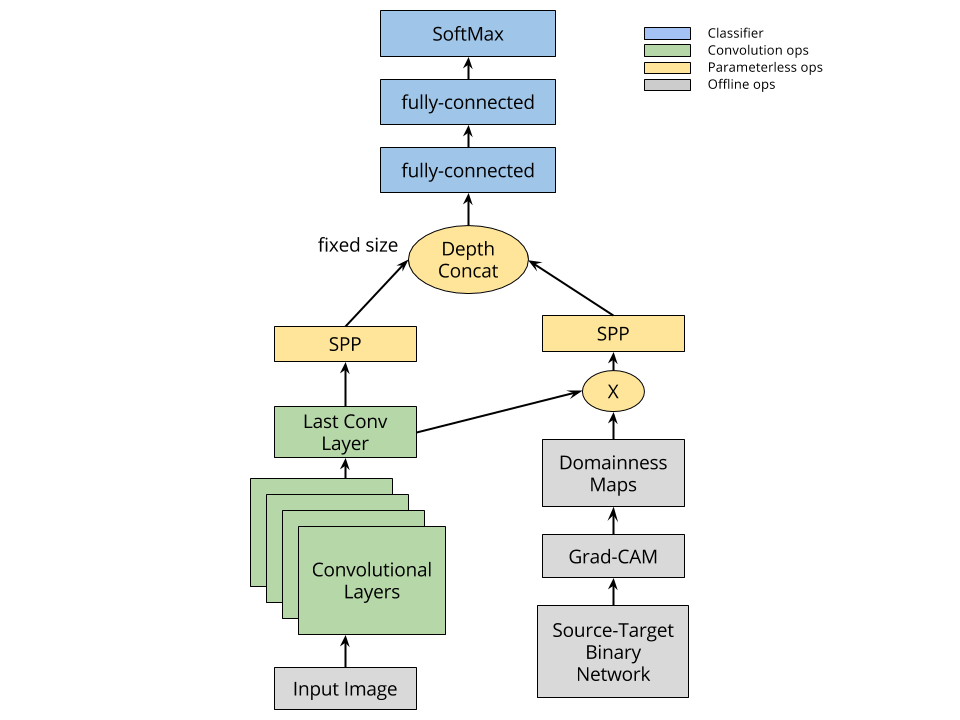
\includegraphics[width=\linewidth]{./img/dmf-architecture.png}
        \caption{Local Adaptive CNN.}\label{fig:dmf-architecture}
    \end{figure}

\end{document}
